\section{Test GUI}

As a means to express the movement recognition of the trained regressors, a test GUI has been implemented to confirm that the regressors are trained accordingly and translate to a specific direction. Furthermore, the test GUI serves as a digital way to test the system before moving on the controlling the JACO robotic arm. 

\begin{figure}[H]
	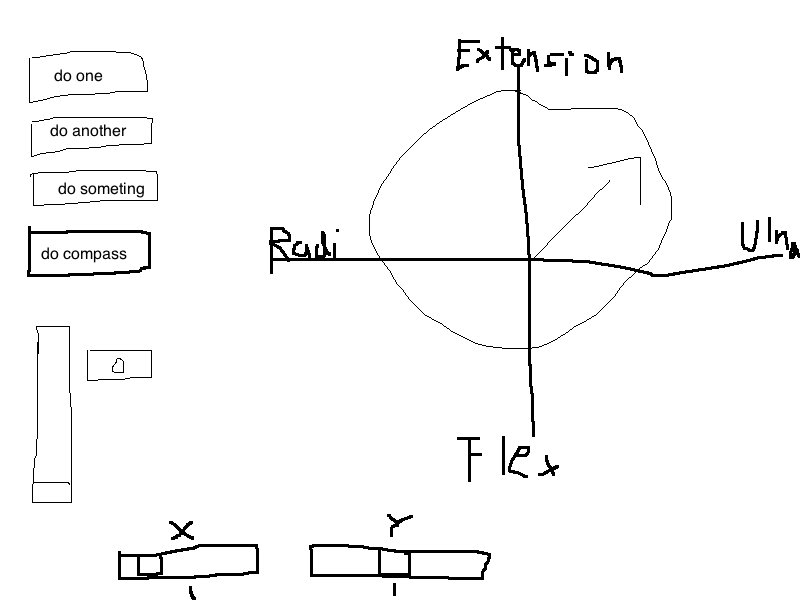
\includegraphics[width=.4\textwidth]{figures/GUI/GUI_test.png}  %<--but is not needed.
	\caption{The compass plot shows the movement and intensity of the EMG, as recognised by the regressor, by arrow direction and length. The test GUI is implemented in the same GUI as the training GUI and will change the plot type once the correct button is pressed.}
	\label{fig:testGUI}
\end{figure}

As seen in \figref{fig:testGUI} the test GUI consists of a compass-like plot with captions for the four movements in four different direction. The compass-plot will illustrate the performed movement by an arrow pointing in the direction of the movement with the intensity of the movement shown as the length of the arrow. The compass-plot have been made so the directions are intuitive in relation to performed movements of the hand, with the palm of the hand facing down as starting point. This is not necessary according to Ison et al. \cite{Ison2016}, as non-intuitive control schemes are not a barrier in learning proper control of prosthetics. The control scheme might change when adapting to system for control of the JACO robotic arm. Sensitivity sliders are implemented in the GUI to enable fine tuning of the intensity to make valid plotting of the arrow in the (X,Y) directions, in case the regressor values are too small to make a proper plot. 
The compass plot will continuously update to plot the direction of the movement and intensity. 